\question The figure below shows the six equally likely values of the 
random pair $(X, Y)$. Specify the functions of:
\begin{itemize}
    \item $L[Y\mid X]$
    \item $E(X\mid Y)$
    \item $L[X\mid Y]$
    \item $E(Y\mid X)$
\end{itemize}

%begin{figure}
%\centering
\begin{center}
    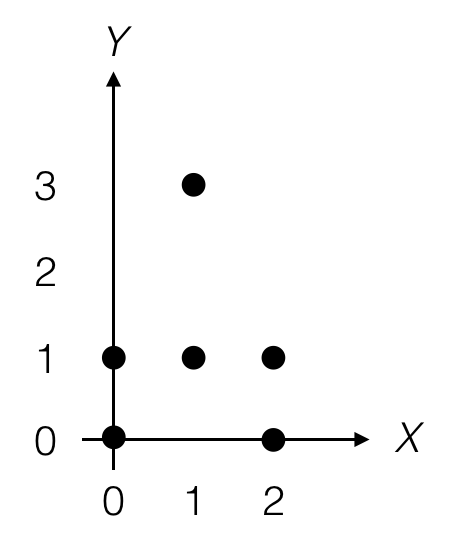
\includegraphics[width=5cm]{find_from_graph.jpg}
\end{center}

\begin{solution}
Let's calculate some useful properties of the distribution first and 
then see how we can use them to calculate the estimates.

\begin{align*}
    |\Omega| = 6 &\implies P[\text{one point}] = \frac{1}{6} \\
    \E(X) &= 0\left(\frac{2}{6}\right) + 1\left(\frac{2}{6}\right) + 
    2\left(\frac{2}{6}\right) \\
    &= 1\\
    \E(Y) &= 0\left(\frac{2}{6}\right) + 1\left(\frac{3}{6}\right) + 
    30\left(\frac{1}{6}\right) \\
    &= 1\\
    \E(XY) &= 0\left(\frac{3}{6}\right) + 1\left(\frac{1}{6}\right) + 
    2\left(\frac{1}{6}\right) + 3\left(\frac{1}{6}\right) \\
    &= 1\\
\cov(X,Y) &= 0 \implies \mathrm{L}[Y|X] = E(Y)
\end{align*}

\begin{itemize}
\item $L[Y\mid X]$: Using the LLSE formula: $\mathrm{L}[Y \mid X] = 
\mathrm{E}[Y] + \frac{\mathrm{Cov}(X,Y)}{\mathrm{Var}(Y)} 
(Y-\mathrm{E}[Y]) = \mathrm{E}[Y]$. Therefore $\boxed{L[Y\mid X] = 1}$

\item $E[X\mid Y]$: Notice the symmetry across $X=1$. For all 
values of $y$, $E[X|Y=y]$ is the same; therefore $\boxed{E[X|Y] = 
E[X] = 1}$. 

\item $L[X\mid Y]$: The MMSE estimator for $X$ given $Y$ is a 
linear function, therefore $\boxed{\mathrm{L}[X\mid Y] = 
\mathrm{E}[X\mid Y] = 1}$

\item $E[Y\mid X]$ For this one we can't make use of symmetry or 
directly apply what we calculated above. We must go back to the 
definition of conditional expectation. We can calculate 
$\mathrm{E}[Y\mid X=x]$ for every point $x$, and that entirely 
defines the expression:
\begin{equation*}
    \mathrm{E}(Y\mid X=x) = 
    \begin{cases}
    \frac{1}{2} \quad\text{if $x = 0$} \\
    2 \quad\text{if $x = 1$} \\
    \frac{1}{2} \quad\text{if $x = 2$}
    \end{cases}
\end{equation*}
The above equation is sufficient, but we can go further by 
realizing that these points are part of a flipped absolute value 
function centered around $x=1$: $\boxed{\mathrm{E}[Y\mid X] = 
\frac{-3}{2} |X-1| + 2}$. Indeed, this is not linear, which is 
why $\mathrm{L}[Y\mid X] \neq \mathrm{E}[Y\mid X]$. 
\end{itemize}
 

 
\end{solution}